Les diagrammes de séquences systèmes réalisés durant l'étape
de conception du bureau distribué sont représentés dans cette 
partie. Il y en a un par cas d'utilisation. 
Ils sont tous représentatifs de la phase de conception du projet
mais ils pourront etre corrigés si les technologies utilisées
varient d'ici l'étape de développement.

\section{Se connecter au bureau distribué}

Ce premier diagramme de séquence système relate le cas d'utilisation
1, qui consiste en la connexion d'un utilisateur au bureau distribué.

\begin{figure}[h!]
	\centering
	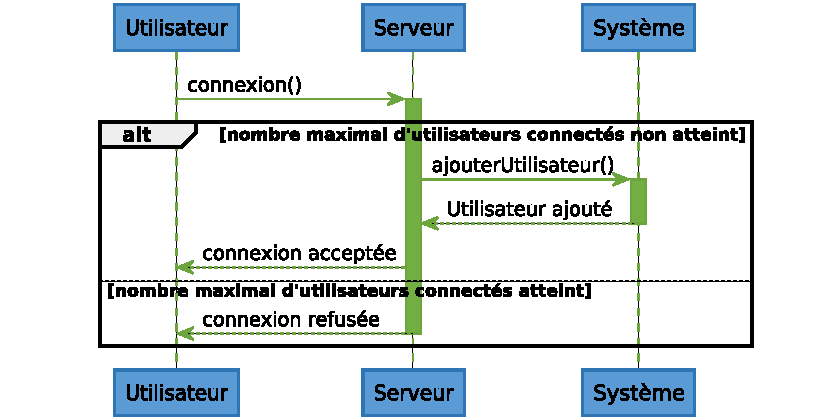
\includegraphics[scale=0.3]{diagrammes/dss1.pdf}
	\caption{\color{green}Diagramme de Séquence Système, cas 1 (mis à jour)\color{black}}
\end{figure}

\section{Ouvrir une fenêtre}

Ce second diagramme de séquence système relate le cas d'utilisation
2, qui consiste en l'ouverture par un utilisateur d'une nouvelle 
fenetre (widget).

\begin{figure}[h!]
	\centering
	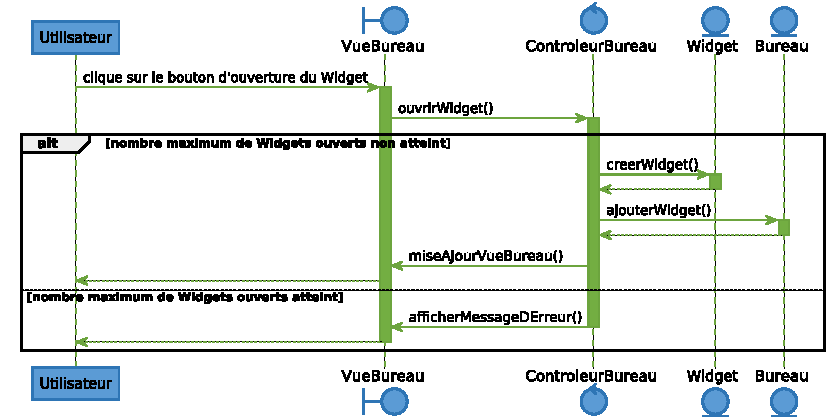
\includegraphics[scale=0.5]{diagrammes/dss2.pdf}
	\caption{\color{green}Diagramme de Séquence Système, cas 2 (mis à jour)\color{black}}
\end{figure}
\newpage
\section{\color{red}{Saisir une opération (Supprimmé)}}

\color{red}{}Ce troisième diagramme de séquence système relate le cas d'utilisation
3, qui consiste en la saisie d'une opération par l'utilisateur dans la 
calculatrice.\color{black}

\begin{figure}[h!]
	\centering
	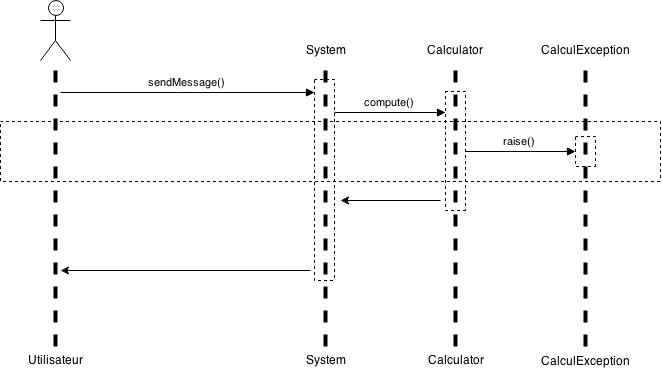
\includegraphics[scale=0.4]{diagrammes/DSS3.jpg}
	\caption{\color{red}{Diagramme de Séquence Système, cas 3}}
\end{figure}

\section{Regarder des photos}

Ce quatrième diagramme de séquence système relate le cas d'utilisation
4, qui consiste à regarder des photos dans le widget galerie.

\begin{figure}[h!]
	\centering
	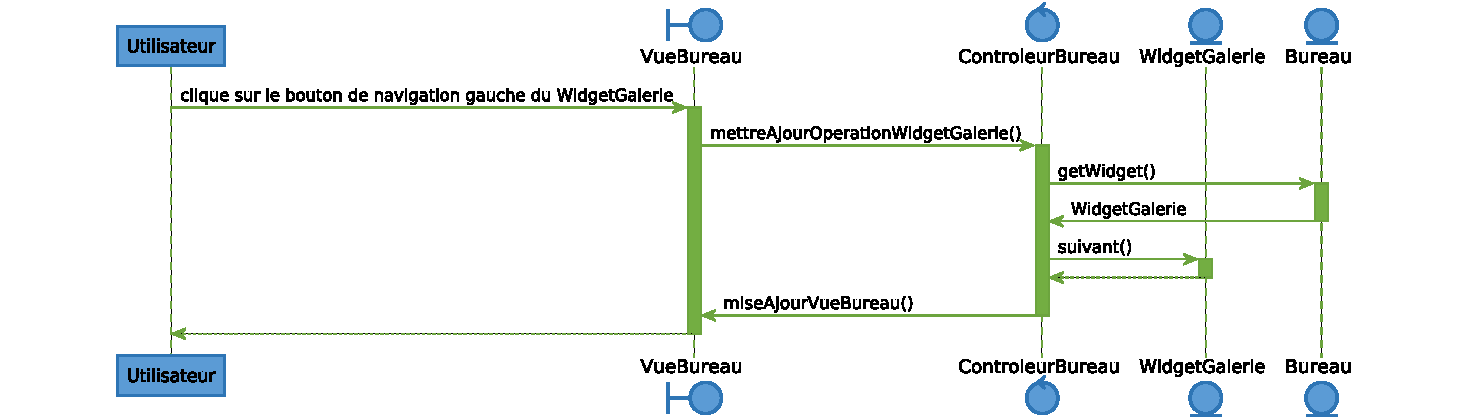
\includegraphics[scale=0.48]{diagrammes/dss4.pdf}
	\caption{\color{green}Diagramme de Séquence Système, cas 4 (mis à jour)\color{black}}
\end{figure}
\newpage

\section{Quitter le bureau virtuel}

Enfin, le dernier diagramme de séquence système relate le cas d'utilisation
5, qui consiste à se déconnecter du bureau virtuel.

\begin{figure}[h!]
	\centering
	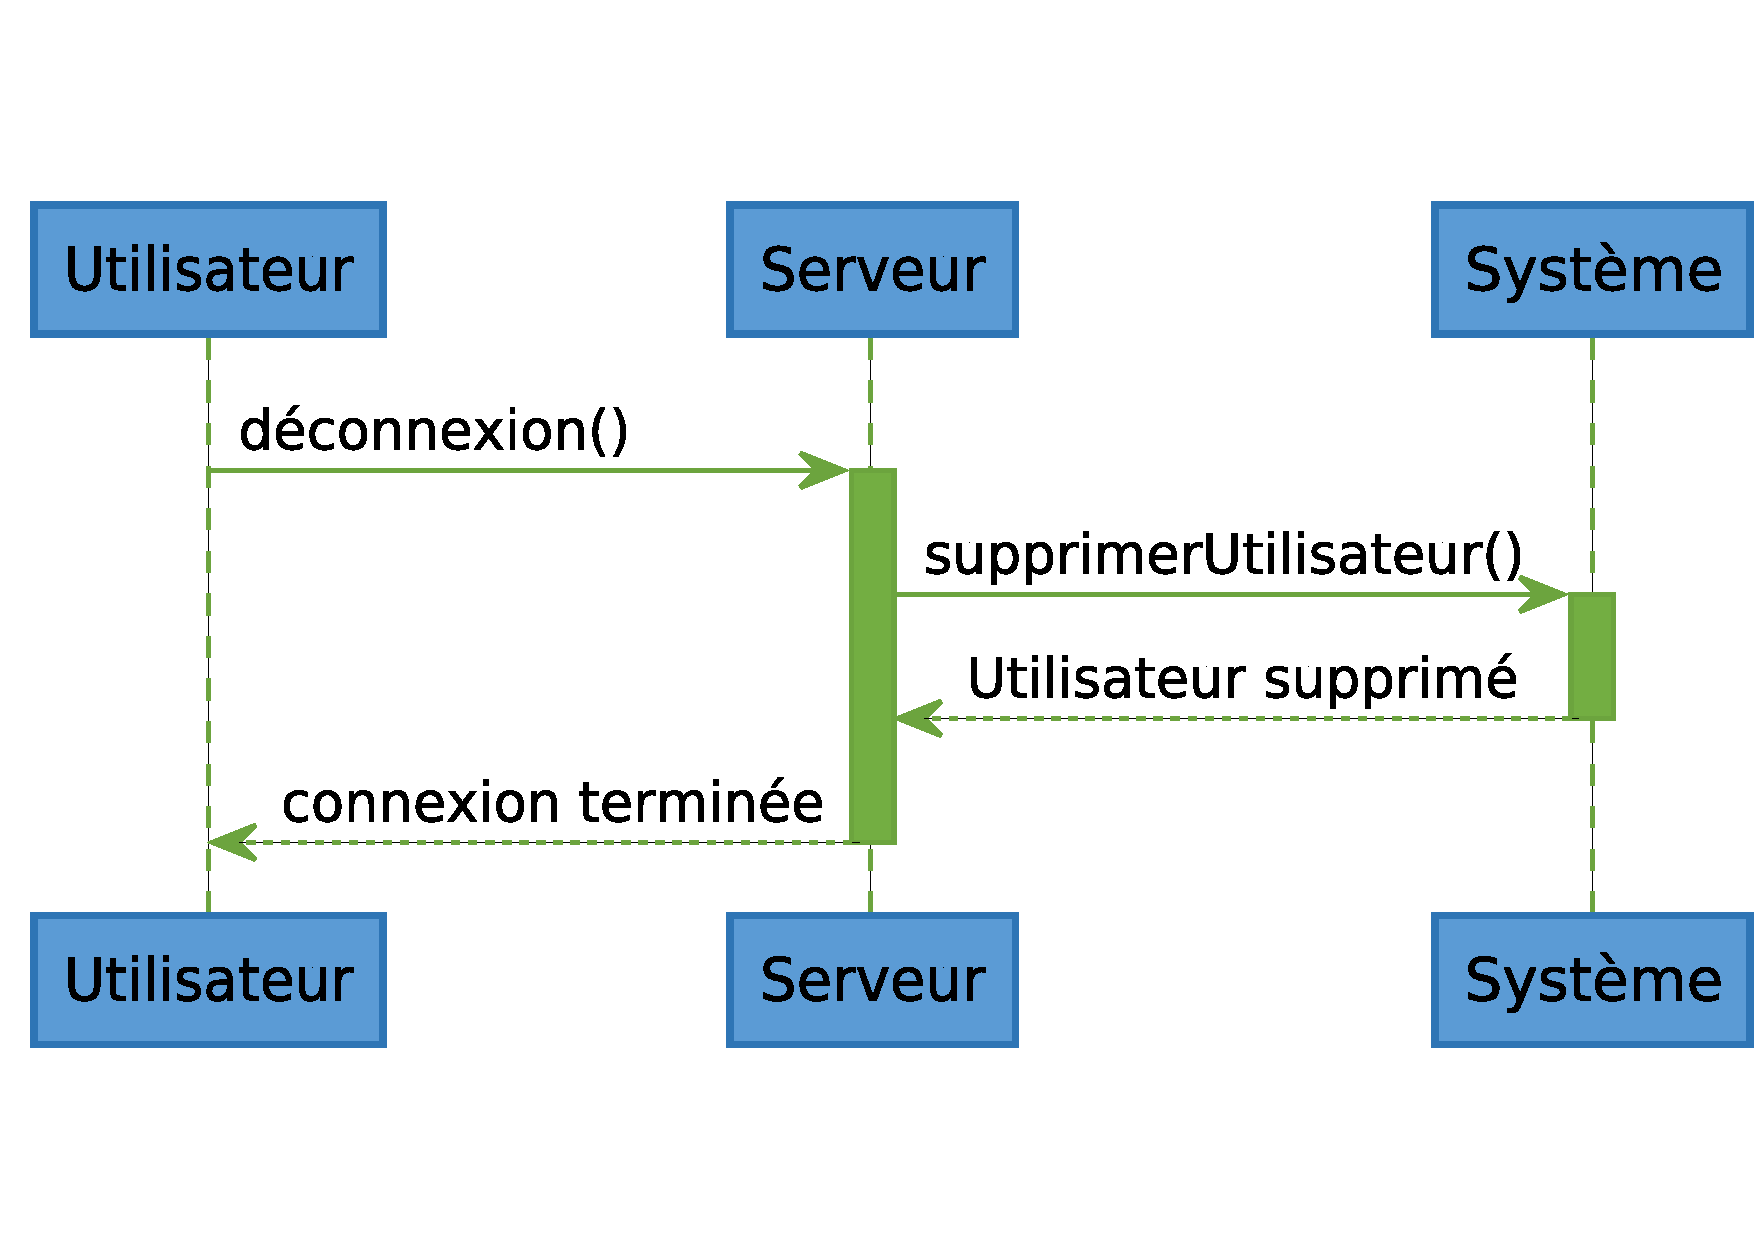
\includegraphics[scale=0.4]{diagrammes/dss5.pdf}
	\caption{\color{green}Diagramme de Séquence Système, cas 5 (mis à jour)\color{black}}
\end{figure}
